\section{Ejercicio 8}

En este ejercicio se busca resolver el problema del ejercicio 3 aplicando una capa intermedia de 100 neuronas con la función de activación \textbf{tanh}.
El grafo computacional correspondiente a este problema es:
\begin{figure}[H]
    \centering
    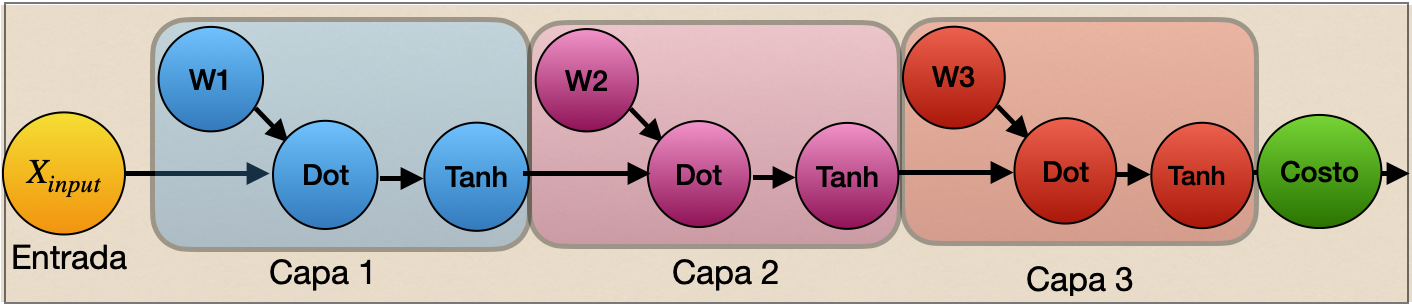
\includegraphics[height=1.5in]{image/EJ8.png}
    \caption{Grafo computacional del ejercicio 8}
    \label{fig:my_label}
\end{figure}


Para comenzar, se cargaron los datos de CIFAR-10 y se creó la estructura solicitada de dos capas con 100 neuronas en la primera capa (original del problema 3), 100 neuronas en la segunda capa (agregada en este problema) y 10 neuronas en la capa de salida.
Nuevamente los datos fueron reacondicionados para expresar la clase de cada imagen como un vector que contiene un 1 en la posición de la clase correcta y el resto de los elementos 0.

Se inicializa la red neuronal con el siguiente fragmento de código:
\begin{verbatim}
# Creo la NN vacía:
model = models.Network()
# Creo la primera capa densa
model.add(layers.Dense(units=100, activation=activations.Sigmoid(), 
input_dim=np.prod(x_train.shape[1:]), factor=1e-2))
# Creo la segunda capa densa:
model.add(layers.Dense(units=100, activation=activations.Sigmoid(), factor=1e-3))  
# Creo la tercera capa densa:
model.add(layers.Dense(units=10, activation=activations.Linear(), factor=1e-2))
# se entrena la NN:
model.fit(x_train, y_train, test_data=test_data, epochs=100, loss=losses.MSE(), 
opt=optimizers.BGD(lr=1e-4, bs=64), name=problem_name, reg=regularizers.L2(lam=1e-3)) 
\end{verbatim}
De acá se ve que se le pasan todos los hiperparámetros del problema al momento del entrenamiento de la red. Se compararon los casos en que la función de costo es MSE, SVM y CCE y se obtuvo la siguiente gráfica:

\begin{figure}[H]
    \centering
    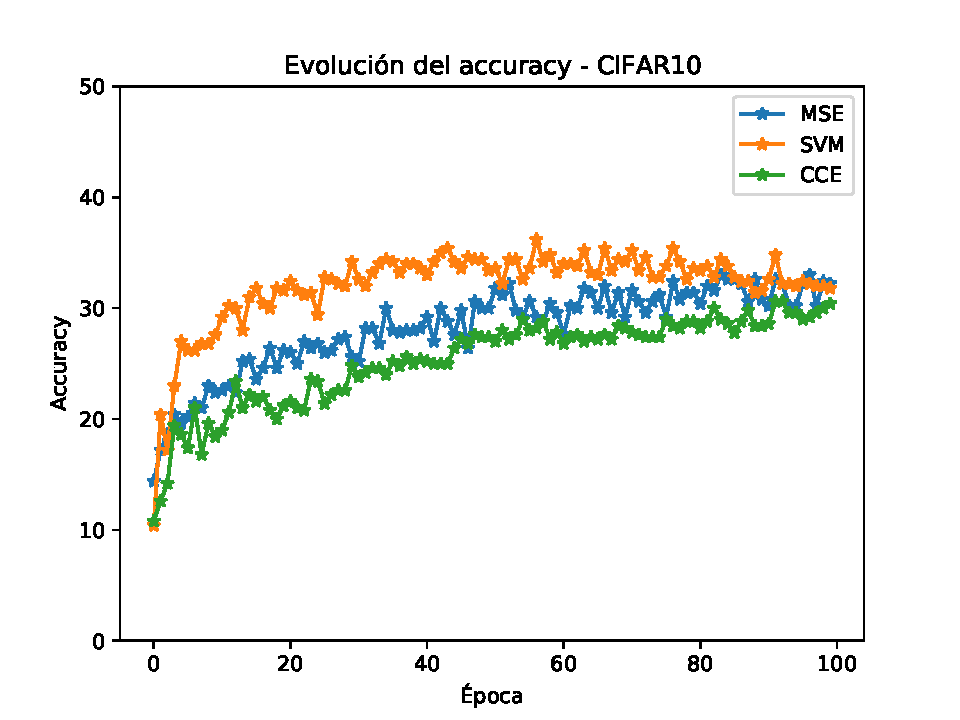
\includegraphics[width=0.45 \textwidth]{image/EJ8_Comparacion.pdf}
    \caption{Accuracy vs. Época del ejercicio 8. Se muestran los resultados de haber usado las funciones de costo MSE, SVM y CCE.}
    \label{fig:my_label}
\end{figure}

Las figuras de abajo muestran los resultados obtenidos para el problema 3 de este trabajo práctico:
\begin{figure}[H]
     \centering
     \begin{subfigure}[b]{0.45\textwidth}
         \centering
         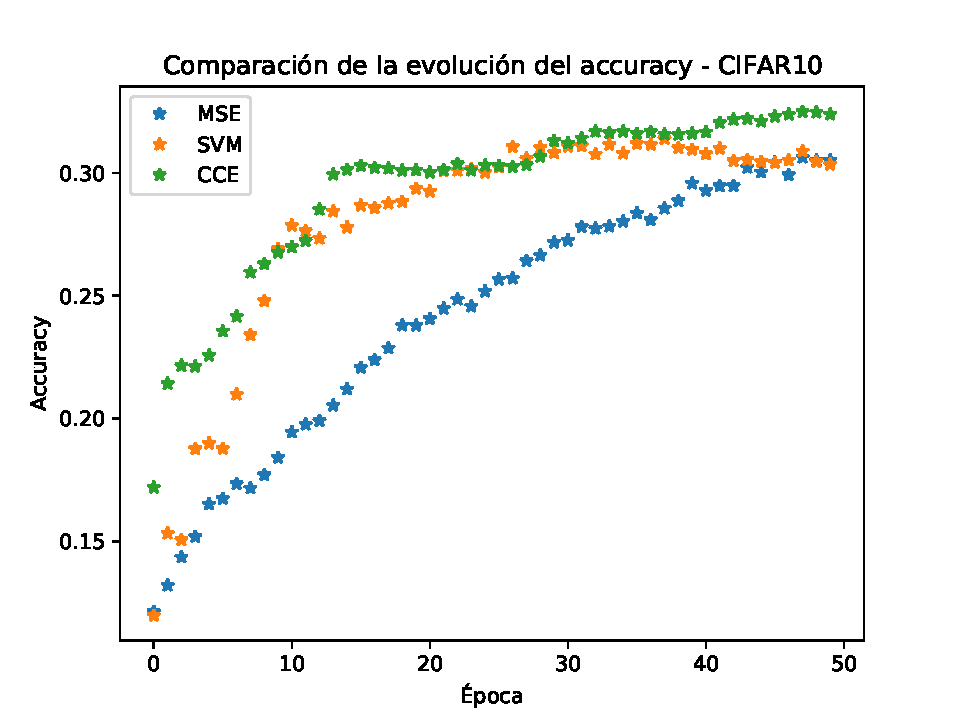
\includegraphics[width=\textwidth]{image/EJ3comparacion2.pdf}
         \caption{Accuracy para el problema 3 del TP2 usando las funciones de costo MSE, SVM y CCE}
         \label{fig:acc6a}
     \end{subfigure}
    \label{fig:ej3_TP2}
\end{figure}

y los resultados del ejercicio 5 del TP1:
\begin{figure}[H]
     \centering
     \begin{subfigure}[b]{0.45\textwidth}
         \centering
         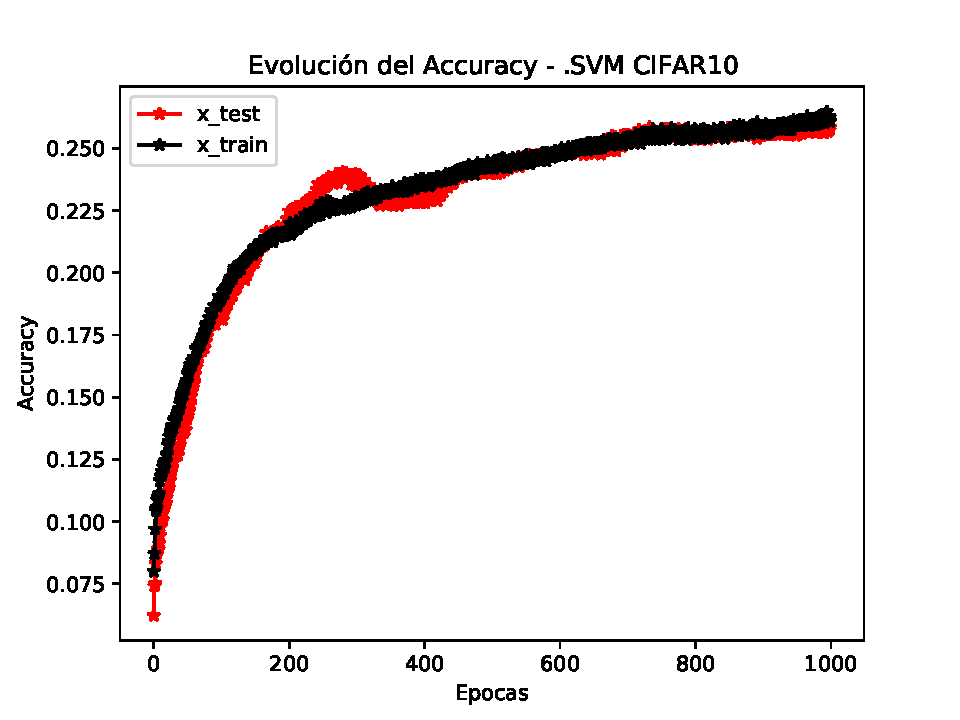
\includegraphics[width=\textwidth]{image/AccuracySVM CIFAR10.pdf}
         \caption{Accuracy para el problema 5 del TP1 usando la función de costo SVM}
         \label{fig:acc6a}
     \end{subfigure}
     \hfill
     \begin{subfigure}[b]{0.45\textwidth}
         \centering
         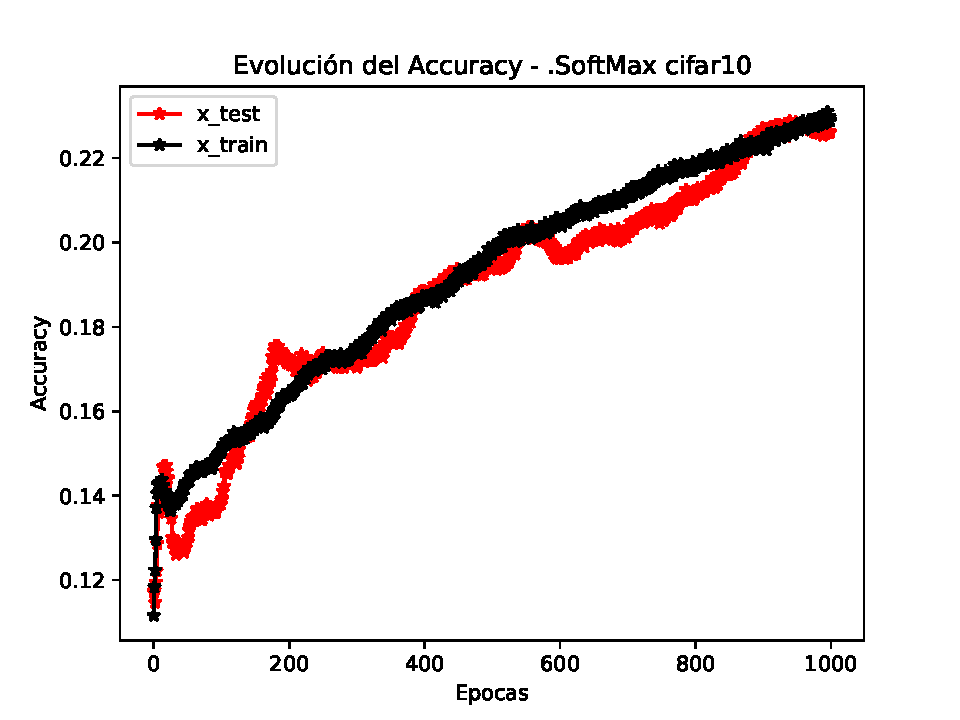
\includegraphics[width=\textwidth]{image/AccuracySoftMax cifar10.pdf}
         \caption{Loss para el problema 5 del TP1 usando la función de costo CCE}
         \label{fig:loss6a}
     \end{subfigure}
        \caption{Resultados obtenidos del ejercicio 5 del TP1 donde no se utilizaban capas ocultas intermedias}
        \label{fig:ej5_TP1}
\end{figure}

Para el problema 8 se usaron 2 capas ocultas de 100 neuronas y una capa de salida de 10 neuronas, para el problema 3 de este trabajo práctico se usó una arquitectura de una capa oculta densa de 100 neuronas y una capa de salida de 10 neuronas y para el problema 5 del TP1 no se usó ninguna capa oculta y la salida tiene una sola neurona.
De comparar los cuatro gráficos, el resultado más llamativo es la cantidad de épocas necesarias para entrenar las redes. Para el ejercicio 8 y 3 se ve que con 50 épocas se alcanza un 'estacionario' mientras que para la arquitectura usada en el problema 5 del TP1 se requieren al menos 500 épocas de entrenamiento para lograr el 'estacionario'.
En cuanto a las precisiones alcanzadas, en el ejercicio 8 se alcanzó una precisión máxima de 33\% para MSE, SVM y CCE, para la arquitectura de solo 2 capas del problema 3 se alcanzaron precisiones de 33\% para el CCE y de 30\% para SVM y MSE. Finalmente para la arquitectura de solo una capa de salida con una neurona (problema 5 del TP1) se alcanzaron despues de 1000 épocas, precisiones del orden de 25\% para SVM y de 23\% para CCE.

En todos los casos se utilizaron 5000 datos para el entrenamiento y los hiper parámetros se ajustaron un poco tratando de que sean lo más parecidos posibles para esta comparación.

En conclusión, se pudo observar el efecto 'acelerador' que tiene la incorporación de capas ocultas con una gran cantidad de neuronas frente a arquitecturas más sencillas como las del problema 5 del TP1. Además de requerir menos épocas y menos tiempo de ejecución, también se logra aumentar la precisión alcanzada por los métodos.
